% One source thumbnail and two reading paths per teaching page.
\clearpage
\begingroup
\newcounter{courseslide}
\newenvironment{slidenotes}[3]{%
  \clearpage
  \begin{center}#3\end{center}\vspace{-2mm}
  \refstepcounter{courseslide}
  \subsection*{Slide #1. #2}\label{slide-#1}
  \addcontentsline{toc}{subsection}{Slide #1. #2}
  \small
}{\par}
\newcommand{\biopath}{\par\smallskip\textbf{Biomedical and imaging path}\par\nobreak}
\newcommand{\sharedpath}{\par\medskip\textbf{Shared interpretation}\par\nobreak}
\newcommand{\comppath}{\par\medskip\textbf{Computational path}\par\nobreak}

\begin{slidenotes}{01}{From brains to models}{
\includegraphics[width=.64\linewidth]{figures/talk/slide-01.png}}
\biopath
What does it mean when a machine outlines the same lesion as a radiologist? The clinician relates contrast to anatomy, disease history and the person's circumstances. A model could reproduce the contour using a narrower cue. Distinguish the observed agreement, the proposed mechanism and the consequence of using the contour. More reproducible measurement can be useful before a treatment benefit has been demonstrated.

\textbf{Exercise and result.} Choose a lesion-follow-up task. Explain in ordinary language what the contour means, what might mislead it and what a patient would need from its use.
\comppath
\textbf{Define the objects.} Let $X$ be the set of admissible inputs and $Y$ the set of possible outputs. The notation $f:X\to Y$ means that a system assigns one output $f(x)$ to each input $x$. Let $g:X\to Y$ be another such system. Compare them on a test set $D=\{x_1,\ldots,x_n\}$ of $n>0$ cases:
\[
A_D(f,g)=\frac{1}{n}\sum_{i=1}^n\mathbf1[f(x_i)=g(x_i)].
\]
\textbf{Read the equation.} The index $i$ labels a case. The indicator $\mathbf1[\cdot]$ is one if the statement in brackets is true and zero otherwise. The summation counts agreements; division by $n$ gives their fraction. Six agreements among eight cases give $A_D=6/8=0.75$. This number is dimensionless and lies between zero and one.

\textbf{Interpretation and exercise.} Even $A_D=1$ means agreement only on the tested cases. For $X=\mathbb R$, $Y=\mathbb R$ and $D=\{0,1\}$, construct two functions agreeing on $D$ but differing at $x=2$. State what the new case rules out and why it still does not identify internal mechanisms. \coursenotebook{00_intro_timeline.ipynb}{Notebook 00} connects this distinction to Marr's levels.
\sharedpath
The clinical account identifies why the task matters; the counterexample establishes why matching answers cannot identify the process producing them.
\end{slidenotes}

\begin{slidenotes}{02}{A learning programme}{
\includegraphics[width=.64\linewidth]{figures/talk/slide-02.png}}
\biopath
What would you need to understand before relying on an output in your field? Start with an observable phenomenon: a growing lesion, a false-positive screen or a convincing but incorrect report. Describe what is seen, what is inferred and what action might follow. An image boundary, an explanation of disease and a decision have different purposes.

\textbf{Exercise and result.} Predict a result verbally before opening a notebook. After running it, explain a surprise to a colleague using biological or clinical concepts and name an observation that could resolve it.
\comppath
\textbf{Define the objects.} Inputs $x$ belong to a space $\mathcal X$ and targets $y$ to $\mathcal Y$. An architecture supplies a family $f_\theta:\mathcal X\to\mathcal Y$, indexed by parameters $\theta$. A loss $L(\hat y,y)$ assigns a numerical penalty to prediction $\hat y$ against target $y$. For $n$ observed pairs $(x_i,y_i)$, distinguish
\[
\widehat R_n(\theta)=\frac1n\sum_{i=1}^n L(f_\theta(x_i),y_i),
\qquad R_P(\theta)=\mathbb E_{(X,Y)\sim P}[L(f_\theta(X),Y)].
\]
\textbf{Read the equations.} The first quantity is average loss on the observed sample; the hat marks an estimate. The second is expected loss for cases drawn from population distribution $P$. Here uppercase $X,Y$ denote random quantities. Expectation $\mathbb E$ means an average over their possible values, weighted by probability. Fitting chooses $\hat\theta\in\arg\min_\theta\widehat R_n(\theta)$: a parameter value achieving the smallest sample loss.

\textbf{Interpretation and exercise.} For zero--one loss, a wrong prediction costs one and a correct prediction zero; risk is an error probability. Give two possible populations compatible with the same finite sample but giving a fixed predictor different risks. Explain why minimizing the observed average does not establish performance in every population.
\sharedpath
The two routes start with different questions and converge on a claim with an explicit purpose, observable result and boundary of inference.
\end{slidenotes}

\begin{slidenotes}{03}{Biological brains across scales}{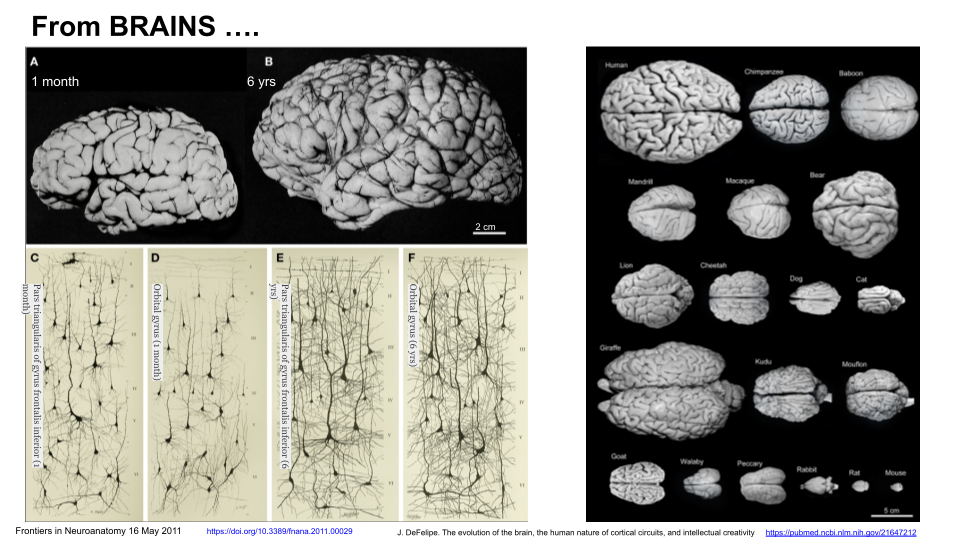
\includegraphics[width=.64\linewidth]{figures/talk/slide-03.png}}
\biopath
How do cellular organisation and whole-brain form relate to an imaging observation? The slide spans developmental drawings and mammalian brains. Respect the scale bars: drawing size does not determine biological size, and visible branching alone does not measure intelligence. An MRI voxel combines signals from many components; different microscopic changes can have similar macroscopic appearances.

\textbf{Exercise and result.} Describe one contrast directly supported by the image. Then propose a cellular explanation and the additional measurement needed to distinguish it from another explanation.
\comppath
\textbf{Define the objects.} Let $s\in\mathbb R^p$ describe a microscopic state and $x\in\mathbb R^m$ its measured image features. The measurement model is
\[
x=H(s)+\epsilon.
\]
The map $H$ translates state into observations; $\epsilon$ represents measurement error in the same units as $x$. The notation $\mathbb R^p$ means a vector with $p$ real-valued components. If $H$ is linear, it is an $m\times p$ matrix, and a vector $v$ in its null space satisfies $Hv=0$.

\textbf{Read the consequence.} Linearity gives $H(s+v)=Hs+Hv=Hs$. A nonzero invisible change $v$ can therefore alter the underlying state without altering the noiseless observation. For example, $H(s_1,s_2)=s_1+s_2$ maps both $(1,2)$ and $(2,1)$ to 3. Non-uniqueness occurs even before noise is added.

\textbf{Interpretation and exercise.} Add a measurement of the first component and recover both components in this example. State which assumption makes that recovery possible. In \coursenotebook{03_bio_vs_artificial.ipynb}{Notebook 03}, separately identify architecture, encoding and update rule: changing them together leaves their individual effects unresolved.
\sharedpath
Biological scale gives the observation meaning; the measurement map explains why one observation may support several underlying states.
\end{slidenotes}

\begin{slidenotes}{04}{Architectures encode choices}{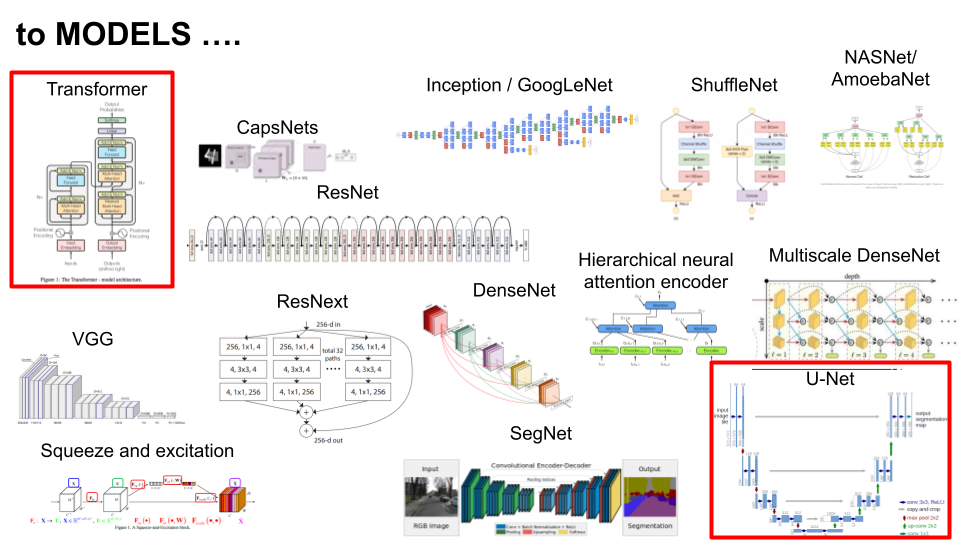
\includegraphics[width=.64\linewidth]{figures/talk/slide-04.png}}
\biopath
Why does a segmentation task need a different organisation from a whole-image classification task? A contour must preserve location and boundaries; a diagnosis-related score may summarize the image. U-Net combines spatial scales, while Transformers combine representations through attention \citep{ronneberger2015,vaswani2017}. Ask which anatomical relationships and image contrasts the output must retain.

\textbf{Exercise and result.} Explain how a system could perform well on large lesions yet miss small ones. Identify the clinical observation that an average score would conceal.
\comppath
\textbf{Define the arrays.} For image height $H$, width $W$ and $C$ measured channels, a segmenter maps $f_\theta:\mathbb R^{H\times W\times C}\to[0,1]^{H\times W}$. Its output $p_i$ is a score at pixel $i$; a binary mask uses $m_i=\mathbf1[p_i\geq\tau]$ for threshold $\tau$. A score in $[0,1]$ requires calibration evidence before being interpreted as an event probability.

For $n$ tokens, each query and key has $d_k$ components and each value has $d_v$. Thus queries $Q$ and keys $K$ have shape $n\times d_k$, while values $V$ have shape $n\times d_v$. One attention operation is
\[
A=\operatorname{softmax}(QK^\top/\sqrt{d_k}),\qquad Z=AV.
\]
\textbf{Read the operations.} Transposition $K^\top$ exchanges rows and columns; $QK^\top$ is an $n\times n$ matrix. Dividing by $\sqrt{d_k}$ scales its dot-product scores. For scaled score $s_{ij}$, softmax sets $A_{ij}=e^{s_{ij}}/\sum_{r=1}^n e^{s_{ir}}$: exponentiate and divide by the row total. Each row therefore sums to one. Multiplication by $V$ makes each row of $Z$ a weighted combination of value vectors, giving shape $n\times d_v$.

\textbf{Interpretation and exercise.} Keep $A$ fixed and replace $V$ by $2V$. Calculate the new $Z$ and explain why weights alone do not determine the output. Trace the operations in \coursenotebook{01_tiny_transformer.ipynb}{Notebook 01} or \coursenotebook{09_segmentation_reflection.ipynb}{09}.
\sharedpath
Anatomical requirements motivate a design; formal dimensions and counterexamples establish what the design actually constrains.
\end{slidenotes}

\begin{slidenotes}{05}{Four questions about intelligence}{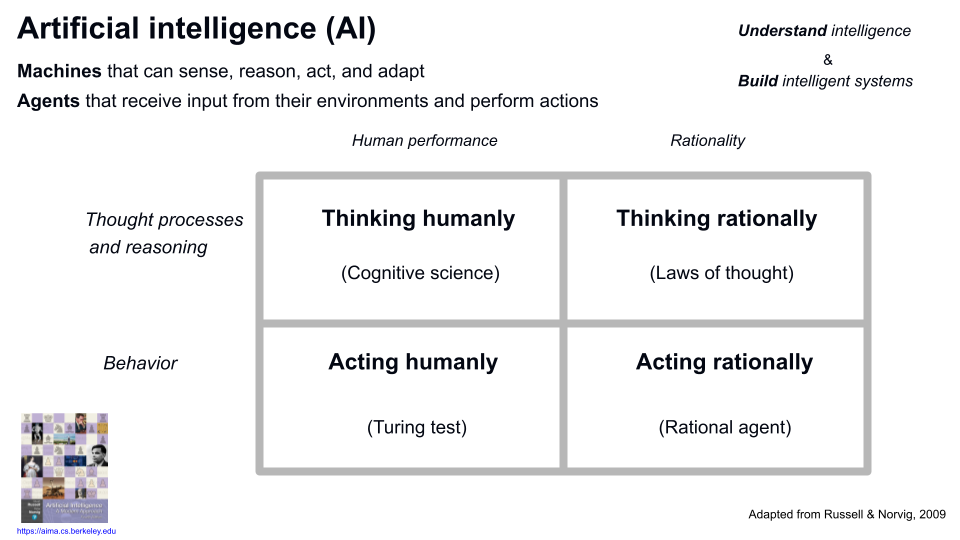
\includegraphics[width=.64\linewidth]{figures/talk/slide-05.png}}
\biopath
What kind of success is claimed? The four views separate human-like thought and action from formally rational thought and action. Agreement with historical prescribing could reproduce a systematic mistake. A logically valid argument can start from an incorrect clinical premise. A beneficial action also depends on the person's priorities.

\textbf{Exercise and result.} Place four questions about one diagnostic decision into the grid. Explain what observations each needs and why the same answer could satisfy one question while failing another.
\comppath
\textbf{Define distinct criteria.} For $n>0$ cases indexed by $i=1,\ldots,n$, let $\hat y_i$ be a model's answer and $h_i$ a human answer. Agreement is $A=n^{-1}\sum_i\mathbf1[\hat y_i=h_i]$. In formal reasoning, $\Gamma\vdash\phi$ means that conclusion $\phi$ can be derived from premises $\Gamma$ using the chosen rules; this does not assert that the premises describe the patient correctly.

For action $a\in\mathcal A$, outcome $y\in\mathcal Y$ and stipulated utility $U(a,y)$, a rational-action criterion is
\[
a^*(x)\in\arg\max_{a\in\mathcal A}
\sum_{y\in\mathcal Y}U(a,y)P(Y=y\mid x).
\]
\textbf{Read the equation.} Conditional probability $P(Y=y\mid x)$ weights each possible outcome after observing $x$. Summing utility times probability gives expected utility. The operator $\arg\max$ returns the maximizing action, not the utility value; $\in$ allows more than one action to tie. The displayed sum assumes a discrete outcome set.

\textbf{Interpretation and exercise.} Give two policies whose agreement and expected utility rank them differently. Supply the probabilities and utilities and calculate both rankings. \coursenotebook{04b_four_views_of_AI.ipynb}{Notebook 04b} organizes these evaluation questions; agreement, derivability and utility are different mathematical targets.
\sharedpath
The clinical route distinguishes meanings of success; the calculation shows that the corresponding objectives can disagree.
\end{slidenotes}

\begin{slidenotes}{06}{Embodiment, judgment and collaboration}{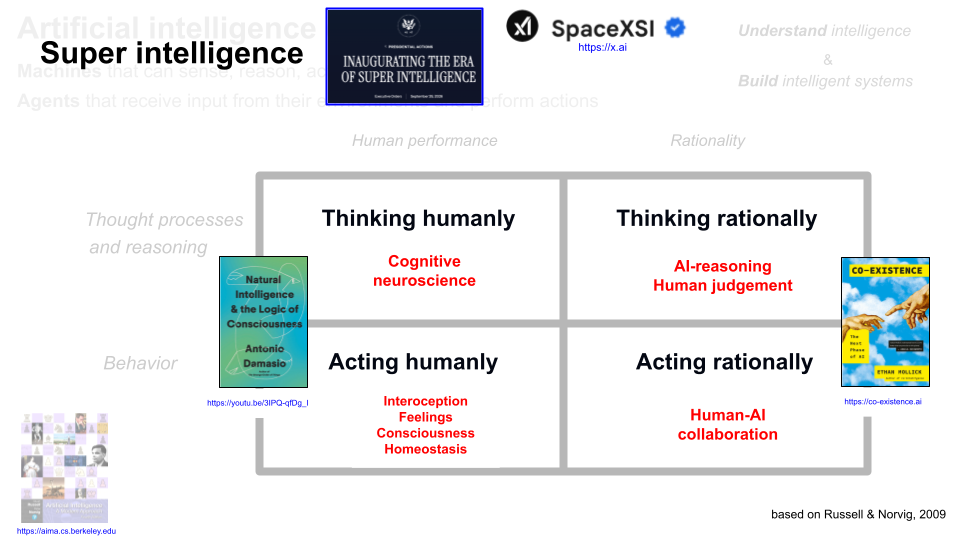
\includegraphics[width=.64\linewidth]{figures/talk/slide-06.png}}
\biopath
Why does bodily regulation matter to accounts of cognition? Interoception concerns signals about internal condition; homeostasis concerns maintaining physiological variables within viable ranges. Hunger, pain and fatigue connect perception to biological needs. Their role motivates hypotheses about embodied understanding without providing a sufficient test for consciousness \citep{seth2013,sethbayne2022}.

\textbf{Exercise and result.} Explain how fatigue could change a person's choice even when the external image is identical. Identify a bodily observation and an alternative explanation for the behaviour.
\comppath
\textbf{Define a feedback system.} At discrete step $t$, let $s_t$ be the system state, $o_t$ its observation, $a_t$ its action and $w_t$ an external disturbance. A controller uses policy $\pi$, possibly with internal memory $m_t$:
\[
o_t=H(s_t),\qquad a_t=\pi(o_t,m_t),\qquad
s_{t+1}=F(s_t,a_t,w_t).
\]
\textbf{Read the loop.} The observation map $H$ supplies information, the policy selects an action, and transition rule $F$ determines the next state. The subscript $t+1$ means the next update, not a derivative. The set $\mathcal V$ contains states declared viable for this model. Invariance means: starting in $\mathcal V$, every allowed disturbance and the specified policy keep the next state in $\mathcal V$.

\textbf{Example and exercise.} For dimensionless $s_{t+1}=s_t+a_t+w_t$, choose $\mathcal V=[-1,1]$. With full observation, unlimited actions and $a_t=-s_t$, the next state is $w_t$; hence $|w_t|\leq0.2$ guarantees invariance. Now limit $|a_t|\leq0.5$ and allow $|w_t|\leq0.6$. Exhibit a starting state and disturbance that break the guarantee. This establishes a functional control property, not a criterion for experience; see Appendix C of the \coursepaper{paper}.
\sharedpath
Biological regulation explains a meaningful need; the formal controller identifies a testable functional property without equating it with experience.
\end{slidenotes}

\begin{slidenotes}{07}{What a Turing-like test measures}{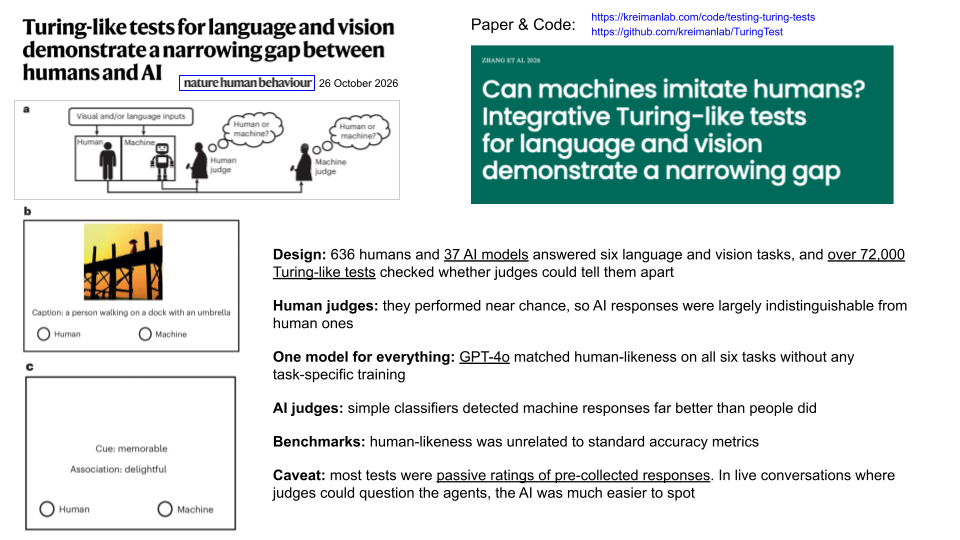
\includegraphics[width=.64\linewidth]{figures/talk/slide-07.png}}
\biopath
What does a person judge in a Turing-like comparison? The cited study's 636 contributors, 37 models and 72,191 judgments concern a specified comparison of human and model responses \citep{zhang2026turing}. Fluency, topic and conversational expectations can affect resemblance. Being difficult to distinguish in that setting does not establish the biological process behind an answer.

\textbf{Exercise and result.} Explain how a fluent scan explanation might appear human while omitting uncertainty important to a patient. Propose a comprehension observation distinct from a resemblance judgment.
\comppath
\textbf{Define one judgment.} Let $T_j\in\{0,1\}$ record item $j$'s true source, with 1 meaning human and 0 model. Judge $i$ supplies classification $J_{ij}$ using the same labels. Correctness is the indicator $Z_{ij}=\mathbf1[J_{ij}=T_j]$. If $\mathcal I$ is the set of $N$ recorded judge--item pairs, estimated accuracy is
\[
\hat a=\frac1N\sum_{(i,j)\in\mathcal I}Z_{ij}.
\]
\textbf{Read the uncertainty.} For $N$ independent, identically distributed Bernoulli judgments, each with success probability $a$, $\operatorname{Var}(\hat a)=a(1-a)/N$. Variance measures spread over repetitions of the sampling procedure. The assumptions matter: judgments sharing a person or an item can be correlated. Merely counting their rows does not establish independence.

\textbf{Example and exercise.} If one random judgment $Z$ is copied $N$ times, their average is still $Z$, so its variance remains $a(1-a)$, rather than shrinking by $N$. Derive this result. Then identify which repetitions in a proposed study share judges, items or model outputs. State the population to which the resulting estimate is intended to refer.
\sharedpath
The human account explains what resemblance means in context; the sampling model limits the precision and scope of the estimate.
\end{slidenotes}

\begin{slidenotes}{08}{Read results in their time and protocol}{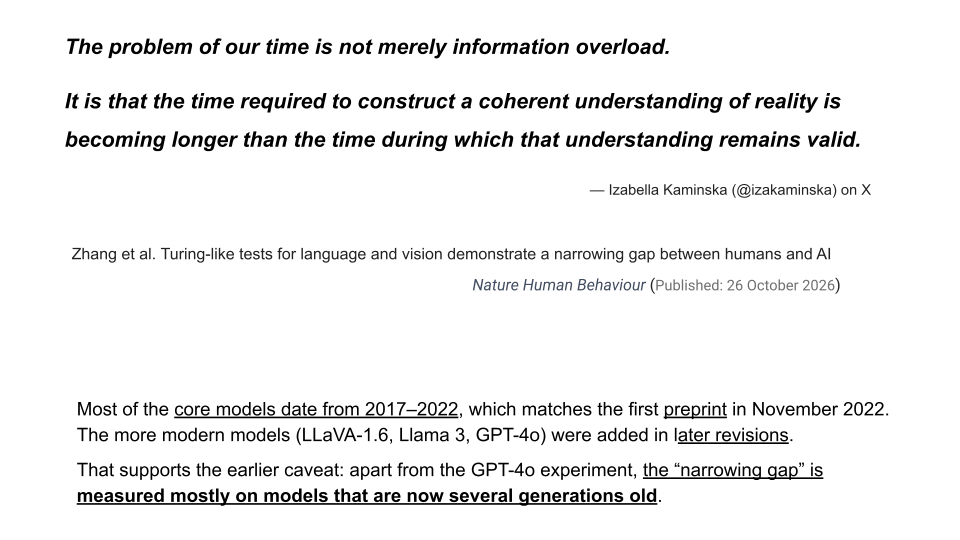
\includegraphics[width=.64\linewidth]{figures/talk/slide-08.png}}
\biopath
How should an impressive result be read when models and protocols evolve? Return to the actual experience being measured: who answered, who judged, what they saw and under which conditions \citep{zhang2026turing}. A later tool-enabled model may support a different workflow from the model in the original comparison.

\textbf{Exercise and result.} Describe a change in presentation that could alter a patient's impression of an answer without improving its clinical content. Explain which observation would detect that difference.
\comppath
\textbf{Define a matched comparison.} A score $S(m,p,D)$ depends on model version $m$, protocol $p$ and evaluation items $D$. To compare versions, keep $p,D$ fixed. For $n>1$ matched items, let $s_{2j}$ and $s_{1j}$ be the two scores on item $j$, measured on the same scale, and define $d_j=s_{2j}-s_{1j}$. Their paired mean difference is
\[
\bar d=\frac1n\sum_{j=1}^n d_j,\qquad
s_d^2=\frac1{n-1}\sum_{j=1}^n(d_j-\bar d)^2.
\]
\textbf{Read the equations.} The bar denotes an average. The second expression, for $n>1$, estimates variation across item differences. If the differences are independent and identically distributed with finite variance, an estimated standard error of the mean is $s_d/\sqrt n$. It has the same units as the score. A positive $\bar d$ favours version 2 only when higher scores mean better performance.

\textbf{Interpretation and exercise.} Distinguish variability across items from variability across repeated generations of one item. Explain why changing the protocol as well as the version no longer isolates a version effect. Construct a scoring-rule change that reverses a ranking while leaving both sets of answers fixed.
\sharedpath
Interpretation depends on the encounter being studied; precise indexing prevents a changing protocol from becoming an unexplained model effect.
\end{slidenotes}

\begin{slidenotes}{09}{Turn a model suggestion into a study}{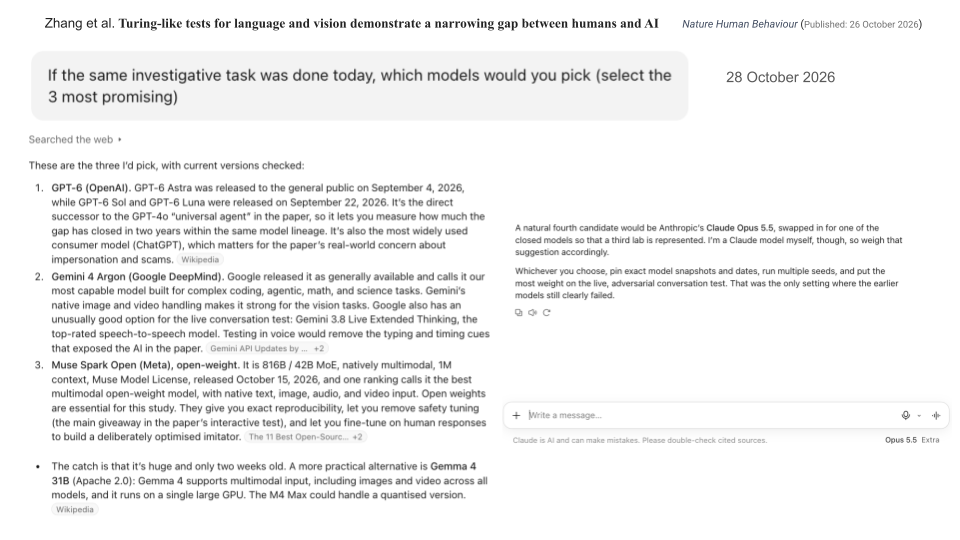
\includegraphics[width=.64\linewidth]{figures/talk/slide-09.png}}
\biopath
How could a suggestion become a meaningful biomedical study? Choose a communication task, such as explaining an uncertain imaging finding. Decide whether the outcome is factual accuracy, patient understanding or trust. These may change differently, and a preference for fluent wording can coexist with poor understanding.

\textbf{Exercise and result.} Draft one comprehension question about a scan explanation and describe an answer that reveals a clinically consequential misunderstanding. Name a population in which the wording should be checked.
\comppath
\textbf{Define the causal question.} Let $a=1$ mean exposure to an AI-assisted explanation and $a=0$ the comparison. For a participant, $Y(1)$ and $Y(0)$ are potential comprehension scores under those two conditions. Parentheses here label hypothetical conditions, not time points. The target average effect is
\[
\Delta=\mathbb E[Y(1)-Y(0)].
\]
\textbf{Read the expression.} Subtract each person's two hypothetical scores, then average over the specified study population. Only one condition is observed for each person. With random assignment, a consistent definition of the intervention and no interference between participants, the difference in assigned-group means estimates this average effect in expectation. It does not reveal each individual's effect.

\textbf{Interpretation and exercise.} Specify the score and its units before collecting data. Compare two strata, such as novice and experienced readers: give group compositions where the aggregate comparison reverses the within-stratum ordering. Calculate both summaries. If one participant answers several questions, distinguish the participant randomized from the repeated measurements analysed. Freeze the scoring rule and evaluation procedure before inspecting their results.
\sharedpath
A clinically meaningful outcome and an identifiable statistical contrast answer complementary parts of the same research question.
\end{slidenotes}

\begin{slidenotes}{10}{From patient data to a useful decision}{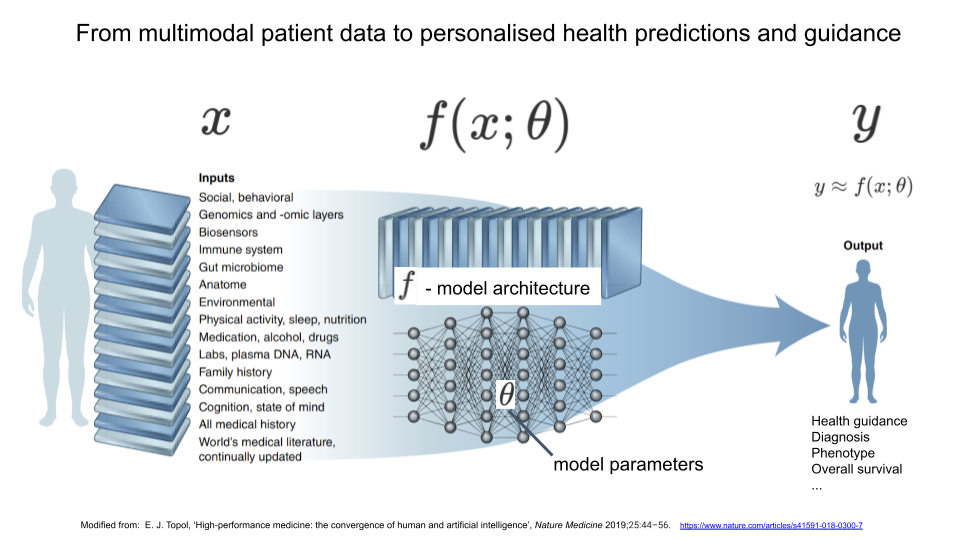
\includegraphics[width=.64\linewidth]{figures/talk/slide-10.png}}
\biopath
How do measurements become a useful decision? A scan, laboratory result and note reflect disease alongside acquisition, referral and recording practices. Their availability also has a time. A result recorded after progression cannot support a prediction made before progression. Risk estimates must then be related to treatment burdens and the person's preferences.

\textbf{Exercise and result.} Trace one input from acquisition to prediction to action. Explain a source of apparent accuracy caused by the care process rather than the intended disease feature.
\comppath
\textbf{Define information and time.} At decision time $t$, $x_{\leq t}$ contains only information available by that time. Let $h>0$ be the forecast horizon and $Y_{t+h}\in\{0,1\}$ the later event. The model estimates $p=P_\theta(Y_{t+h}=1\mid x_{\leq t})$, a number between zero and one. Parameters $\theta$ are fitted earlier; the action policy uses the resulting probability.

For two actions, assign zero cost to correct decisions, positive cost $C_{FP}$ to acting when the event is absent and $C_{FN}$ to not acting when it is present:
\[
L_{\rm act}=(1-p)C_{FP},\qquad L_{\rm wait}=pC_{FN}.
\]
\textbf{Read and rearrange.} Each expected loss is probability times consequence. Acting is preferred when $(1-p)C_{FP}<pC_{FN}$, equivalently
\[
p>\frac{C_{FP}}{C_{FP}+C_{FN}}.
\]
Costs must use the same units; their ratio is dimensionless. At equality the actions tie under these assumptions.

\textbf{Exercise and interpretation.} Put $C_{FP}=1$, $C_{FN}=4$ and calculate the boundary. Explain why a future note included in $x_{\leq t}$ changes the prediction problem. \coursenotebook{15_ppv_and_decisions.ipynb}{Notebook 15} separates this action boundary from the threshold used to classify test scores.
\sharedpath
The clinical account defines the available evidence and meaningful consequences; the decision inequality makes their assumed relationship explicit.
\end{slidenotes}

\begin{slidenotes}{11}{Keep the task fixed across Marr's levels}{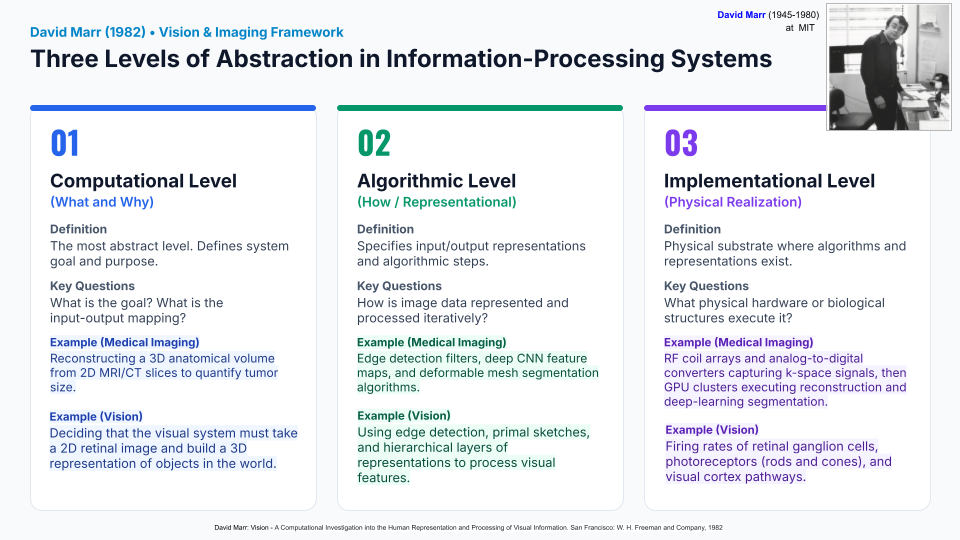
\includegraphics[width=.64\linewidth]{figures/talk/slide-11.png}}
\biopath
What is being explained when a system segments an image? Marr's levels separate purpose, representation and procedure, and physical implementation \citep{marr2010}. For lesion follow-up, the purpose may be reproducible change measurement. A mask is one representation; the scanner, computer and biological visual system realize different processes.

\textbf{Exercise and result.} Explain why identical contours do not establish identical visual recognition. Describe what a clinician's history-taking adds to the purpose of the task.
\comppath
\textbf{Define a spatial representation.} A binary mask $m$ has value $m_i=1$ at a selected voxel and zero elsewhere. Voxel $i$ occupies physical volume $v_i$ in mm$^3$. Summing the selected volumes gives
\[
V(m)=\sum_i v_i m_i.
\]
\textbf{Read the units.} Each mask value is dimensionless, so $V$ is in mm$^3$; divide by 1000 to express it in mL. For 1,000 selected voxels of 2~mm$^3$ each, $V=2,000$~mm$^3=2$~mL. The mapping from image $x$ to mask, $m=f_\theta(x)$, differs from the composed mapping $x\mapsto V(f_\theta(x))$ that retains only volume.

For two masks on the same grid, the triangle inequality gives
\[
|V(m)-V(\tilde m)|\leq\sum_i v_i|m_i-\tilde m_i|.
\]
\textbf{Interpretation and exercise.} Tilde $\tilde m$ names an alternative mask. The right side counts disagreement volume: both omitted and extra selected voxels. Derive the bound and construct equal-volume masks at different locations. Equal summaries do not imply equal representations or algorithms. \coursenotebook{00_intro_timeline.ipynb}{Notebook 00} relates these distinctions to Marr's explanatory levels.
\sharedpath
Clinical purpose chooses what needs explaining; the mappings distinguish an output, its summary statistic and the process that produces it.
\end{slidenotes}

\begin{slidenotes}{12}{Read about AI with an application in mind}{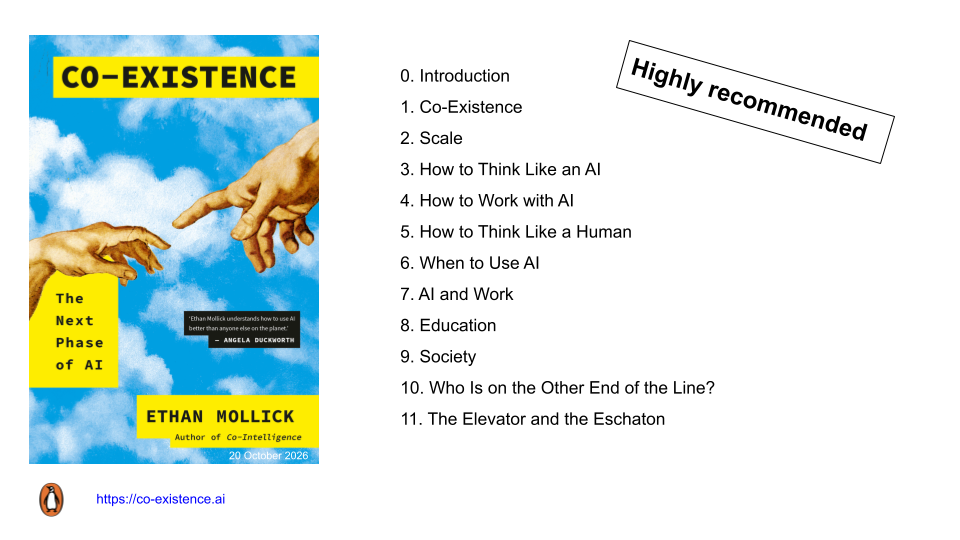
\includegraphics[width=.64\linewidth]{figures/talk/slide-12.png}}
\biopath
How should an appealing AI application be evaluated? The application discussion \citep{mollick2026coexistence} invites a useful question about coexistence with professional work. Begin with the patient's problem and the observed task. A faster draft may still require correction of negation, laterality and uncertainty. An elegant overlay may emphasize an annotation convention rather than a disease boundary.

\textbf{Exercise and result.} Compare one proposed application with the present workflow. Describe a helpful change and a plausible failure in ordinary clinical language.
\comppath
\textbf{Define an evaluation claim.} Specify $(\mathcal X,\mathcal Y,P,L,B)$: input space, target space, evaluation population, loss and baseline procedure. For matched case $i$, let $L_i^{AI}$ and $L_i^B$ be the two losses; the superscripts label procedures, not powers. Define $d_i=L_i^{AI}-L_i^B$. Negative $d_i$ favours AI because lower loss is better.

If the population has groups $g$ with proportions $w_g$, mean loss difference decomposes as
\[
\bar d=\sum_g w_g\bar d_g,\qquad w_g\geq0,\quad\sum_gw_g=1.
\]
\textbf{Read the equation.} Each group mean $\bar d_g$ is weighted by that group's share. For two groups with shares 0.9 and 0.1, differences $-0.1$ and $+0.5$ give $\bar d=-0.04$. Thus the overall average improves while the smaller group worsens. These are constructed loss differences, not study results.

\textbf{Interpretation and exercise.} Recalculate after changing the group proportions. Explain which target population the resulting number describes. Then specify a controlled change to a suspected irrelevant image input, as in \coursenotebook{08_attention_maps.ipynb}{Notebook 08}'s marker replacement. \coursenotebook{11_shortcut_dependence.ipynb}{Notebook 11} changes marker--target association across populations. An average and a feature intervention answer different questions.
\sharedpath
The application is meaningful through its clinical use; the formal claim exposes the population, comparison and error pattern it actually tests.
\end{slidenotes}

\begin{slidenotes}{13}{Preserve the ability to judge}{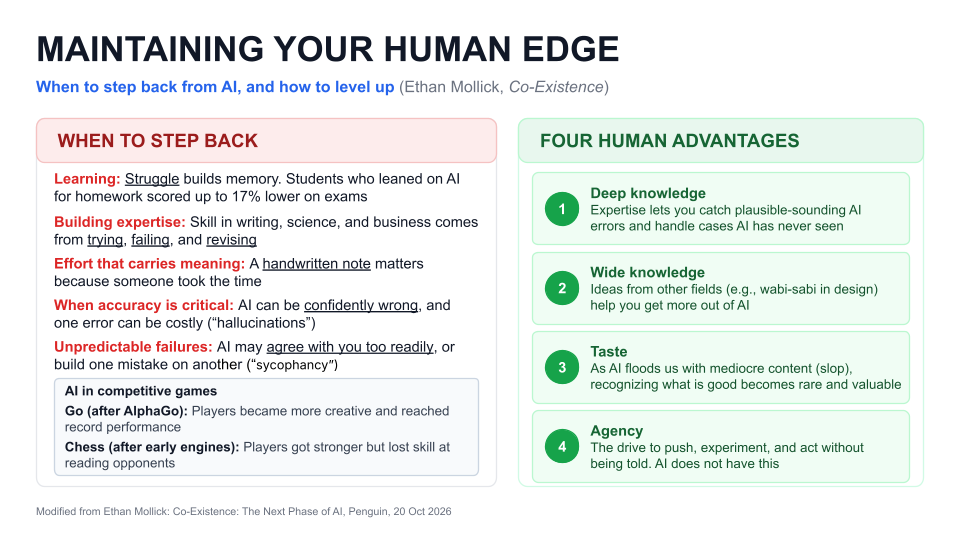
\includegraphics[width=.64\linewidth]{figures/talk/slide-13.png}}
\biopath
How can assistance affect the ability to judge later? Immediate help can reduce effort while changing which skills receive practice. In the cited mathematics study, unrestricted GPT assistance was associated with a 17\% reduction in later unaided performance in that setting \citep{bastani2025learning}. This is a prompt for a biomedical teaching question, rather than an estimate for clinical trainees.

\textbf{Exercise and result.} Explain how accepting a lesion overlay repeatedly could affect later unaided boundary judgments. Propose a teaching activity that requires the learner to explain and check the result.
\comppath
\textbf{Define two outcomes.} Let $S_a$ denote a score obtained with assistance and $S_l$ a later score obtained without assistance. The subscripts name assessment conditions. For assigned groups $A,B$, define
\[
\Delta_a=\bar S_{a,A}-\bar S_{a,B},\qquad
\Delta_l=\bar S_{l,A}-\bar S_{l,B}.
\]
\textbf{Read the contrasts.} A bar means the mean across participants in that group. Both differences compare the same groups, but they concern different outcomes. Neither definition forces the signs to agree. In an invented example, assisted means 0.8 versus 0.6 give $\Delta_a=0.2$, while later means 0.60 versus 0.75 give $\Delta_l=-0.15$.

\textbf{Interpretation and exercise.} If scores are proportions correct, $-0.15$ is a decrease of 15 percentage points. Relative to 0.75, it is a $100(0.60-0.75)/0.75=-20\%$ change. Distinguish these two descriptions and keep the constructed example separate from the cited study. Design a later assessment using new items, without access to the assisted answers, and identify the participant-level comparisons needed to estimate retained performance.
\sharedpath
The learning account explains why retained judgment matters; separate outcomes prevent immediate task success from standing in for later competence.
\end{slidenotes}

\begin{slidenotes}{14}{Map the frontier task by task}{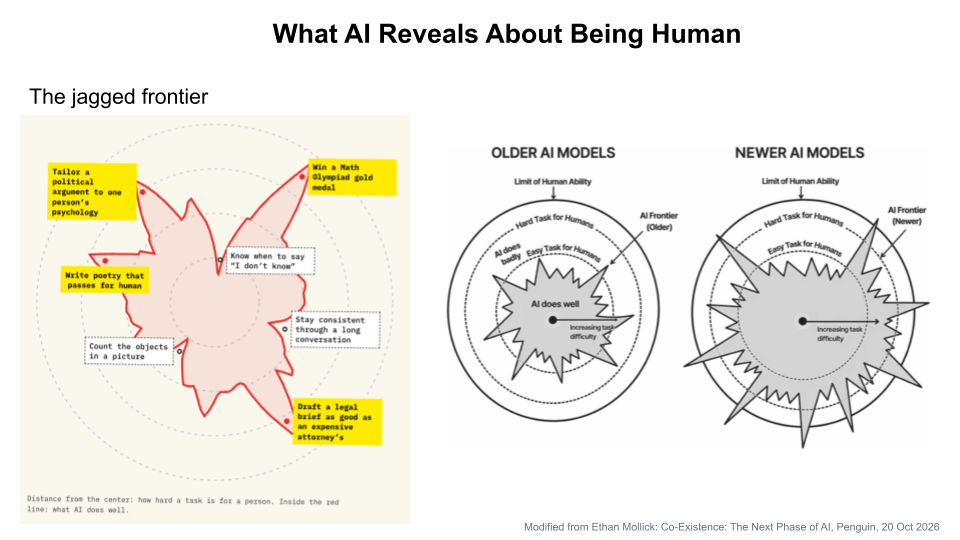
\includegraphics[width=.64\linewidth]{figures/talk/slide-14.png}}
\biopath
Which parts of a task remain dependable when the situation changes? The discussion of an uneven capability frontier \citep{mollick2026coexistence} fits imaging: common anatomy may be handled well while an unusual acquisition or subtle lesion exposes failure. A professional also interprets the consequences of an error for the particular person.

\textbf{Exercise and result.} Describe two tasks that appear similar but need different clinical knowledge. Predict a circumstance in which success on one gives weak reassurance about the other.
\comppath
\textbf{Define risk for a setting.} A fixed predictor $f$ can be evaluated under different joint distributions $P_1,P_2$ of inputs and targets. For discrete inputs and targets,
\[
R_{P_t}(f)=\sum_{x,y}P_t(x,y)L(f(x),y),\qquad t\in\{1,2\}.
\]
\textbf{Read the equation.} The loss at each possible case is weighted by that case's probability in setting $t$. Zero--one loss makes this risk an error probability. Changing the setting can change those weights, or which cases have any probability, without changing $f$.

For a concrete example, let $f(a)=0$, $f(b)=1$ and the true label be 0 at both inputs. If $P_1$ puts all mass at $a$ and $P_2$ all mass at $b$, the risks are zero and one. Perfect performance in the first setting supplies no guarantee for the second without assumptions connecting them.

\textbf{Exercise and interpretation.} In \coursenotebook{11_shortcut_dependence.ipynb}{Notebook 11}, the fixed rule predicts marker $M$. Show that its accuracy is $P(M=Y)$ and its risk $1-P(M=Y)$. Explain which distribution changes and which function stays fixed. A task label alone does not specify that distribution.
\sharedpath
Clinical differences suggest where to test; the counterexample explains why transfer needs stated assumptions and observations.
\end{slidenotes}

\begin{slidenotes}{15}{Specify, inspect, revise and stop deliberately}{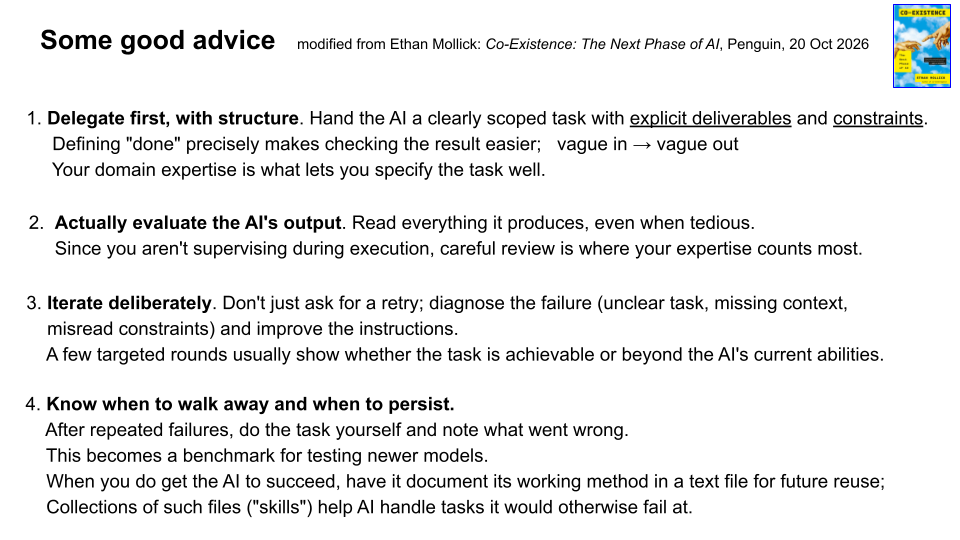
\includegraphics[width=.64\linewidth]{figures/talk/slide-15.png}}
\biopath
When is a model-assisted result ready to use? In a clinical or research explanation, preserving uncertainty can matter as much as fluent wording. A person must judge whether a proposed conclusion fits the observed anatomy, history and limits of the measurement. Repeated revision can improve presentation while leaving an incorrect premise intact.

\textbf{Exercise and result.} Rewrite an uncertain finding for a patient. Explain which words preserve uncertainty and what additional observation would justify a stronger statement.
\comppath
\textbf{Define a procedure.} Let state $q_k$ contain the current draft, sources and check results after iteration $k$. Action $u_k$ could request a revision or run a check. The transition $q_{k+1}=T(q_k,u_k)$ describes how the next state is produced. An acceptance predicate $C(q)\in\{0,1\}$ returns one only when the declared criteria are met.
\[
\tau=\min\{k\in\{0,\ldots,K\}:C(q_k)=1\}.
\]
\textbf{Read the stopping rule.} Here $K$ is a finite iteration budget and $\tau$ the first accepted iteration. If the set is empty, report that acceptance was not reached within the budget; there is no minimum to return. This $\tau$ is a stopping index, distinct from an image threshold using the same Greek letter elsewhere.

\textbf{Interpretation and exercise.} A predicate checking only grammar can accept an unsupported diagnostic statement. Construct that example, then add a criterion comparing the statement with the source findings. Explain why repeating a deterministic check on an unchanged state adds no new evidence about failures that the check does not measure. Acceptance establishes the chosen criteria; it does not establish every possible property of the output.
\sharedpath
Clinical judgment supplies meaningful acceptance criteria; explicit state and stopping rules make the resulting procedure inspectable.
\end{slidenotes}

\begin{slidenotes}{16}{Compartments, anatomy and measurement}{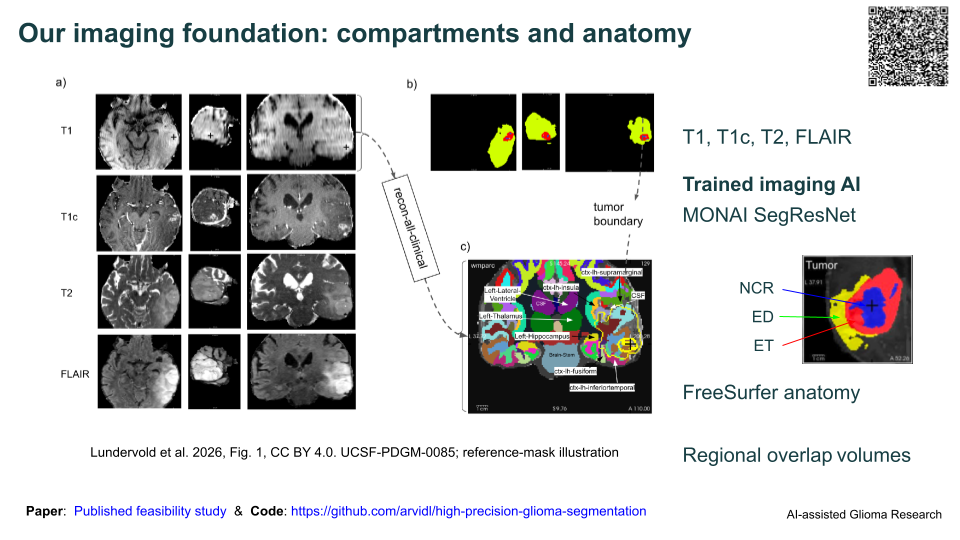
\includegraphics[width=.64\linewidth]{figures/talk/slide-16.png}}
\biopath
What does an anatomical compartment represent? Grey matter, white matter, fluid spaces and tumour-related appearances have different biological meanings. An anatomical phantom supplies geometry, while the lesson assigns transport coefficients and a seed. Those assignments do not turn normal BrainWeb images into measured tumour progression \citep{lundervold2026glioma}.

\textbf{Exercise and result.} Predict how a closed fluid barrier might change spread. Explain why removing a thin barrier by coarse sampling could change the simulated pattern, even if the growth rates are unchanged.
\comppath
\textbf{Define geometry and density.} For voxel index $i=(i_1,i_2,i_3)$, a $4\times4$ affine matrix $A$ converts indices to millimetres:
\[
(x_1,x_2,x_3,1)^\top=A(i_1,i_2,i_3,1)^\top.
\]
The final 1 permits translation as well as rotation and scaling. The upper-left spatial block $A_{3\times3}$ has a determinant giving signed volume scaling. Its absolute value removes the orientation sign, so voxel volume is $v=|\det A_{3\times3}|$ in mm$^3$. Let $u_i=c_i/K$ be density relative to constant carrying capacity $K$, both densities having units cells/mm$^3$.
\[
B=\frac v{1000}\sum_i u_i,\quad
V_\tau=\frac v{1000}\sum_i\mathbf1[u_i\geq\tau],\quad
N=Kv\sum_i u_i.
\]
\textbf{Read the sums.} $B$ weights each voxel by its density fraction; $V_\tau$ counts voxels above threshold $\tau$ equally. Both are in mL; $N$ is a cell count. At 4-mm isotropic spacing, $v=64$~mm$^3=0.064$~mL. A voxel with $u_i=0.25$ contributes 0.016~mL to $B$ and 0.064~mL to $V_{0.2}$.

\textbf{Exercise and interpretation.} Prove $V_{\tau_2}\leq V_{\tau_1}$ for $\tau_2\geq\tau_1$ by comparing the selected sets. Use \coursenotebook{14b_brainweb_growth.ipynb}{Notebook 14b} to separate physical geometry, assigned rates and simulated density.
\sharedpath
Anatomical interpretation and dimensional accounting identify which quantity a coloured compartment can legitimately represent.
\end{slidenotes}

\begin{slidenotes}{17}{Population growth and a mechanistic hypothesis}{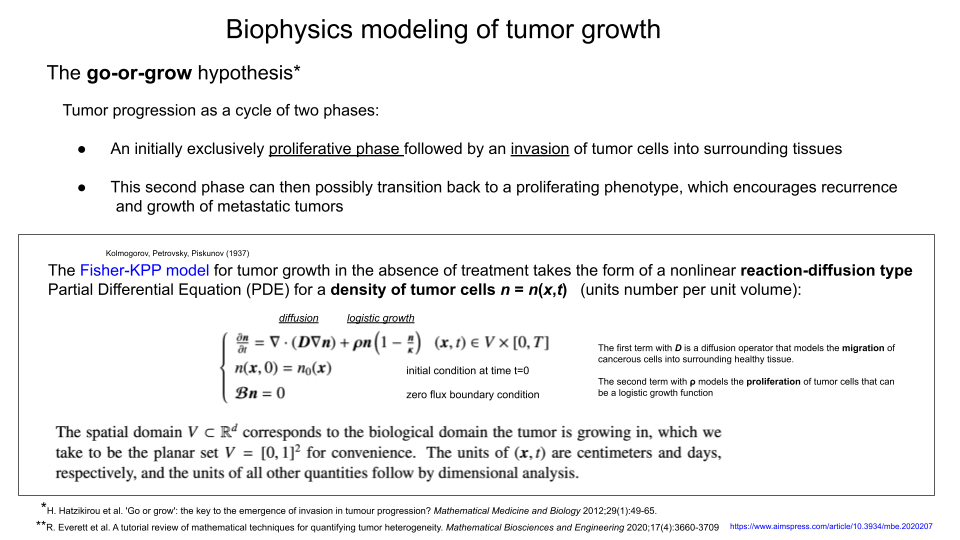
\includegraphics[width=.64\linewidth]{figures/talk/slide-17.png}}
\biopath
How can proliferation and dispersal change a population? Births increase local density; movement redistributes cells. Crowding can limit growth. The go-or-grow hypothesis concerns a further distinction between migratory and proliferative states \citep{hatzikirou2012}; the basic Fisher--KPP equation contains no explicit switching between those states.

\textbf{Exercise and result.} Predict what happens when movement is disabled, then when proliferation is disabled in a closed domain. Explain which observation distinguishes local accumulation from redistribution.
\comppath
\textbf{Define the field.} $c(\mathbf x,t)$ is density at position $\mathbf x$ in tissue domain $\Omega$ and time $t$. Density and capacity $K$ are in cells/mm$^3$, scalar diffusivity $D$ in mm$^2$/day and proliferation rate $\rho$ in day$^{-1}$:
\[
\partial_t c=\nabla\!\cdot(D\nabla c)+\rho c(1-c/K).
\]
\textbf{Read the operators.} $\partial_t c$ is local change per day. The gradient $\nabla c$ points toward increasing density. Cell flux is $\mathbf j=-D\nabla c$; its divergence measures net outward flow, so redistribution contributes $-\nabla\!\cdot\mathbf j$. The final term is logistic proliferation: approximately $\rho c$ at low density and zero at $c=K$.

No flux means $\mathbf n\cdot\mathbf j=0$ at the boundary, with $\mathbf n$ the outward unit normal. Total cells $M=\int_\Omega c\,dV$ then satisfy
\[
\dot M=\int_\Omega\rho c(1-c/K)\,dV.
\]
The integral adds density over physical volume; the dot means a time derivative. Thus $M$ is in cells and $\dot M$ in cells/day.

\textbf{Exercise and interpretation.} Derive the balance and set $\rho=0$ to establish conservation. With $D=0$, verify $c(t)=K/[1+(K/c_0-1)e^{-\rho t}]$ has initial value $c_0>0$. \coursenotebook{13_verified_growth_model.ipynb}{Notebook 13} checks these processes separately.
\sharedpath
The biological route distinguishes the processes; the balance and exact limit establish separate numerical checks for them.
\end{slidenotes}

\begin{slidenotes}{18}{An interactive simulation is an experiment}{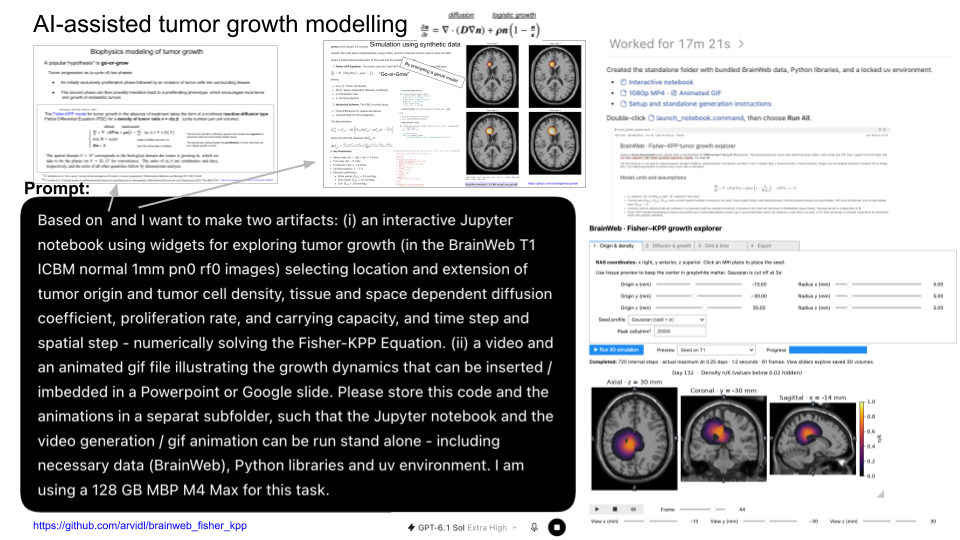
\includegraphics[width=.64\linewidth]{figures/talk/slide-18.png}}
\biopath
How can an interactive simulation become a controlled numerical experiment on a biological model? Begin with \coursenotebook{14d_coupled_tumour_growth.ipynb}{Notebook 14d}'s small CPU preset. Reduced delivery or greater oxygen consumption can slow proliferation and, below a lower threshold, promote loss of viable cells. Necrotic material and a displayed MRI appearance are different concepts.

\textbf{Exercise and result.} Predict where oxygen would first become scarce as the population grows. Change uptake alone, rerun, and explain the viable and necrotic patterns. Then change only time or slice position and describe what the display reveals about the same run.
\comppath
\textbf{Define state and display separately.} Let $U_0=(c_0,z_0)$ specify initial viable and necrotic densities. Parameters $\theta$ include transport, proliferation and oxygen settings. A solution operator $S_\theta$ computes the fields at time $t$:
\[
U_\theta(t)=S_\theta(t;U_0)=(c_\theta(t),z_\theta(t),o_\theta(t)),
\qquad I=H_{\tau,k,j}[U_\theta(t)].
\]
\textbf{Read the composition.} $U_\theta(t)$ denotes whole spatial fields, rather than one voxel. The display operator $H_{\tau,k,j}$ selects field $j$, physical slice $k$ and threshold $\tau$ where applicable; $I$ is the resulting image. The oxygen view uses the tissue mask rather than the density cutoff. Changing the display operator reads the same computed state; changing a model parameter requires solving again.

\textbf{Interpretation and exercise.} Compare uptake $\beta=0$ with $\beta=4$, keeping seed, domain, grid, $D$, $\rho$ and $K$ fixed. Define the difference in total viable cells at a fixed day. Then change only the display threshold and explain why that full-volume count is invariant. In this lesson, changing grid spacing also resamples anatomical barriers; it cannot by itself isolate a time-stepping or display effect.
\sharedpath
A spatial biological prediction becomes a controlled parameter intervention only when state changes and display changes are kept explicit.
\end{slidenotes}

\begin{slidenotes}{19}{From a biological diagram to coupled variables}{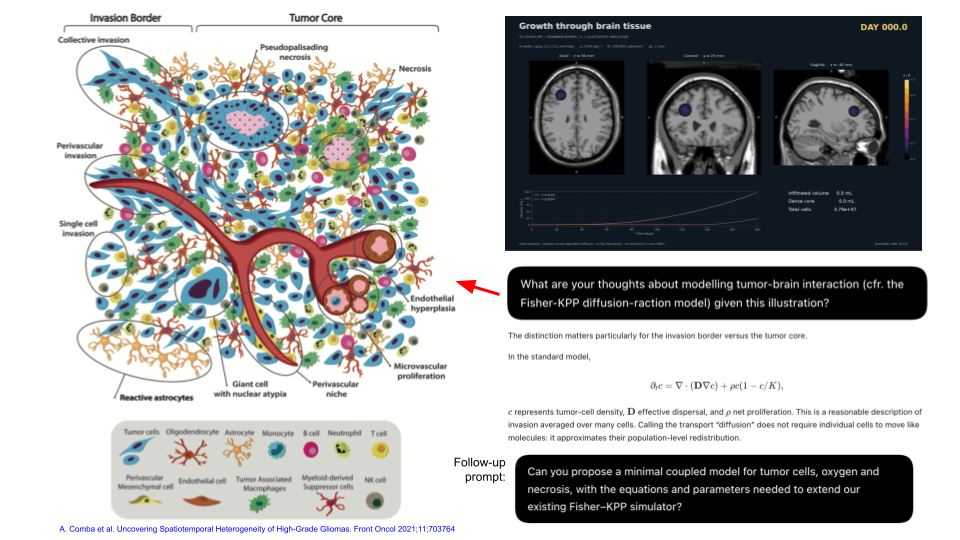
\includegraphics[width=.64\linewidth]{figures/talk/slide-19.png}}
\biopath
Which processes in the glioma diagram need separate state variables? The illustration shows viable tissue, necrotic regions, invasion and vascular relationships \citep{comba2021heterogeneity}. Delivery brings oxygen; consumption removes it. Poorer availability can reduce births before causing death. In the lesson, necrotic material remains in place and occupies capacity; vessels and angiogenesis are omitted.

\textbf{Exercise and result.} Predict where a viable rim and a necrotic core might develop. Explain why a region with fewer viable cells need not contain an equal increase in necrotic material. Distinguish both from an MRI signal.
\comppath
\textbf{Define the compartments.} At position $\mathbf x$ in mm and time $t$ in days, $c(\mathbf x,t)$ is viable density and $z(\mathbf x,t)$ immobile necrotic material, in cell equivalents/mm$^3$. Both are defined on tissue domain $\Omega$; capacity $K$ has the same units. Relative oxygen $o$ is dimensionless, with normal baseline one. In \coursenotebook{14d_coupled_tumour_growth.ipynb}{Notebook 14d}, births $B$ and death transfer $T$ are
\[
B=\rho g(o)c[1-(c+z)/K]_+,\qquad T=\delta h(o)c,
\]
where $[a]_+=\max(a,0)$ prevents negative births; $g,h$ are defined on slide 20. The coupled equations are
\[
\begin{aligned}
\partial_tc&=\nabla\!\cdot(D\nabla c)+B-T,\\
\partial_tz&=T-\lambda_z z,\\
0&=\ell_o^2\Delta o+p(1-o)-\beta(c/K)o,\qquad p=[1+\alpha(c+z)/K]^{-1}.
\end{aligned}
\]
\textbf{Read the terms.} Diffusion redistributes viable cells. Transfer subtracts from $c$ and adds equally to $z$; $\lambda_z z$ clears necrotic material. The zero on the oxygen equation means a quasi-steady balance: spatial smoothing plus delivery minus consumption. Here $\Delta o$ is the Laplacian. The factor $p$ describes delivery, $\alpha$ its suppression by material, $\beta$ oxygen uptake and $\ell_o$ a smoothing length. Proliferation, death and clearance rates $\rho,\delta,\lambda_z$ are in day$^{-1}$, $D$ in mm$^2$/day and $\ell_o$ in mm; $p,\alpha,\beta$ are dimensionless.

\textbf{Exercise and interpretation.} Add the density equations and integrate over a no-flux domain. For $M=\int_\Omega(c+z)\,dV$, derive $\dot M=\int_\Omega B\,dV-\lambda_z\int_\Omega z\,dV$. Explain why death transfer cancels, and why fewer viable cells than in the reference cannot all be counted as necrosis.
\sharedpath
Viable-cell loss relative to the reference combines altered proliferation and death; the total-material balance prevents interpreting every missing viable cell as necrosis.
\end{slidenotes}

\begin{slidenotes}{20}{Compare states with matched displays}{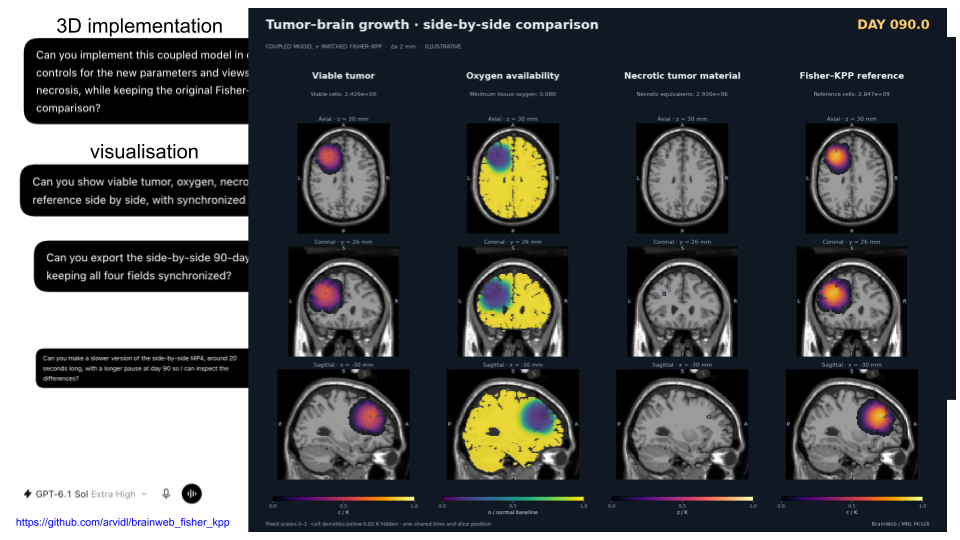
\includegraphics[width=.64\linewidth]{figures/talk/slide-20.png}}
\biopath
What do the four matched views reveal? Read viable tumour, oxygen, necrotic material and the Fisher--KPP reference at the same day and physical location. A viable deficit may reflect fewer births as well as death. Clearance removes necrotic material only if enabled; the presets use $\lambda_z=0$. None of these fields is a measured patient MRI.

\textbf{Exercise and result.} Predict the pattern after disabling oxygen uptake, rerun \coursenotebook{14d_coupled_tumour_growth.ipynb}{14d}, and explain why a difference image alone cannot identify a death rate. Use the trajectories to support the explanation.
\comppath
\textbf{Define the oxygen response.} With dimensionless thresholds $0<\theta_d<\theta_p<1$, the proliferation and death modifiers are
\[
g(o)=\min(1,o/\theta_p),\qquad h(o)=\max(1-o/\theta_d,0).
\]
\textbf{Read the functions.} Proliferation reaches its full rate when $o\geq\theta_p$ and is reduced below it. Death transfer occurs only when $o<\theta_d$. For example, $o=0.15$, $\theta_p=0.3$, $\theta_d=0.1$ give $g=0.5$ and $h=0$: births are reduced without oxygen-induced death.

To establish the zero-uptake limit, set $\beta=0$ and $w=o-1$. Multiply the oxygen equation by $w$, integrate over $\Omega$ and integrate the Laplacian by parts. No-flux boundaries remove the boundary term. With positive perfusion $p$ and $\ell_o>0$, this gives
\[
0=-\ell_o^2\int_\Omega|\nabla w|^2\,dV-\int_\Omega p w^2\,dV.
\]
Both integrals on the right are nonnegative before the minus signs; their sum can vanish only with $w=0$, so $o=1$. Then $g=1$, $h=0$ and, for $z_0=0$, $z$ stays zero. Constant $K>0$, nonnegative $D,\rho$ and $0\leq c_0\leq K$ preserve $0\leq c\leq K$; the clipped birth term then equals Fisher--KPP's logistic term.

\textbf{Exercise and interpretation.} Explain each assumption and match seed, domain, $D$, $\rho$ and $K$ to the reference. Distinguish this continuum argument from the numerical comparison up to solver tolerance.
\sharedpath
The biological prediction and the mathematical limit meet in a strong implementation check; physiological adequacy still needs independent measurements.
\end{slidenotes}

\begin{slidenotes}{21}{Agents produce different kinds of evidence}{
\includegraphics[width=.64\linewidth]{figures/talk/slide-21.png}}
\biopath
What kind of evidence has an agent produced? The four categories distinguish extraction, ranked hypotheses, refined candidates and empirically validated knowledge \citep{primeview2026}. A plausible oxygen-growth explanation is a hypothesis until appropriate observations test it. Repeating the same generated analysis does not create new biological samples.

\textbf{Exercise and result.} Follow a claim from a cited paper to an agent's proposed experiment. Explain which observation could contradict it and what a failed test would mean biologically.
\comppath
\textbf{Define the procedure and its score.} An agent's state $q_k$ can contain a draft hypothesis, retrieved sources and previous tool results. At step $k$, action $a_k$ obtains result $r_k$, and $q_{k+1}=T(q_k,a_k,r_k)$ updates the state. Reproduction requires that trace and a stopping rule, not just the final sentence.

To see selection bias, let $Z_1,Z_2$ be two independent noisy scores, each equally likely to be $-1$ or $+1$. Both have expectation zero. Selecting the larger score gives
\[
P(\max(Z_1,Z_2)=-1)=\tfrac14,\qquad
\mathbb E[\max(Z_1,Z_2)]=(-1)\tfrac14+(+1)\tfrac34=\tfrac12.
\]
\textbf{Read the calculation.} The maximum is negative only when both scores are negative. Three of the four equally likely pairs contain a positive score. The selected result therefore averages above zero even though neither underlying score has a positive expectation.

\textbf{Interpretation and exercise.} Enumerate those four pairs, then define an independent evaluation unavailable during candidate selection. Explain why rerunning an agent on the same observations can assess procedural variability but cannot create independent biological samples. A high selected score and new evidence for a hypothesis are different results.
\sharedpath
Biological evidence supplies a test of the claim; the formal selection example explains why a convincing best run needs an independent evaluation.
\end{slidenotes}

\begin{slidenotes}{22}{Place assistance inside the research design}{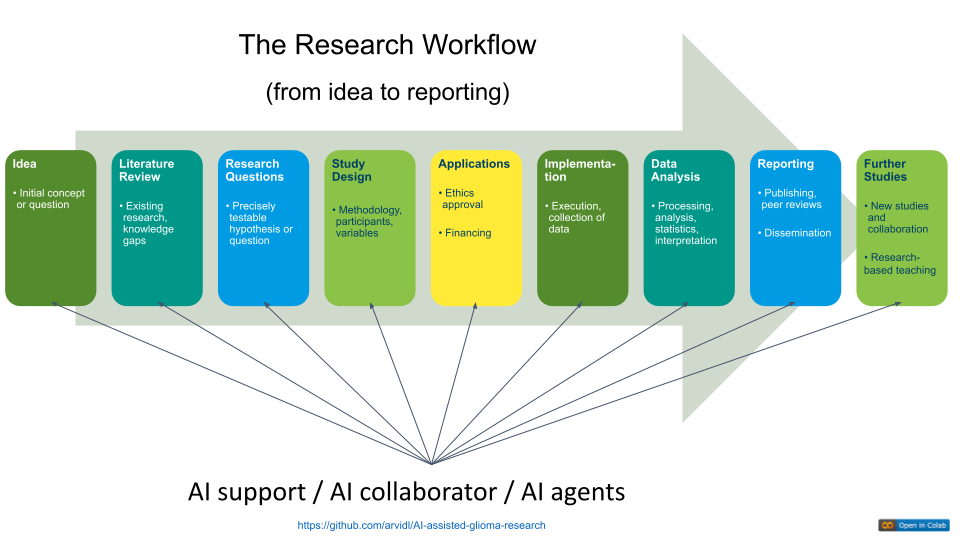
\includegraphics[width=.64\linewidth]{figures/talk/slide-22.png}}
\biopath
Can serial imaging constrain a model well enough to forecast a later observation? Define what the scan measures, how scans are aligned and which change matters. A close fit to earlier images may leave dispersal and proliferation hard to distinguish. Comparison with persistence asks whether the added mechanisms improve prediction.

\textbf{Exercise and result.} Describe an imaging or biological measurement that could separate fast dispersal from fast local proliferation. Explain why forecasting progression does not by itself estimate a treatment effect.
\comppath
\textbf{Define the inverse problem.} In \coursenotebook{14c_growth_parameter_recovery.ipynb}{Notebook 14c}, $\theta=(s,\rho)$ contains a dimensionless diffusivity multiplier and a growth rate in day$^{-1}$. The simulated field $u_\theta=c_\theta/K$ is dimensionless. Observation operator $H$ averages $2\times2\times2$ blocks. For observation time $t_j$ and retained block $i$ in the region of interest (ROI), $y_{j,i}$ is a generated noisy observation. Fit by minimizing
\[
J(\theta)=\frac1{N_{\rm obs}}\sum_{j,i}
\bigl([H u_\theta(t_j)]_i-y_{j,i}\bigr)^2,
\qquad \hat\theta\in\arg\min_{\theta\in\Theta_{\rm grid}}J(\theta).
\]
\textbf{Read the objective.} Square brackets identify block $i$ after averaging. Each residual is predicted minus observed density fraction. $N_{\rm obs}$ counts all included time--block pairs, so $J$ is mean squared error. Only days 20, 40 and 60 enter fitting; day 90 is withheld. The controlled grid $\Theta_{\rm grid}$ contains the generating pair.

\textbf{Exercise and interpretation.} Persistence predicts $\hat y^{\rm pers}_{90,i}=y_{60,i}$. Compare its day-90 residual with $[Hu_{\hat\theta}(90)]_i-y_{90,i}$. Explain why similar early predictions can leave different parameter pairs difficult to distinguish, even when the search returns a precise minimum.
\sharedpath
The biomedical question identifies an informative observation; the objective and held-out comparison define exactly which recovery and forecast claims were tested.
\end{slidenotes}

\begin{slidenotes}{23}{A creative workflow and its provenance}{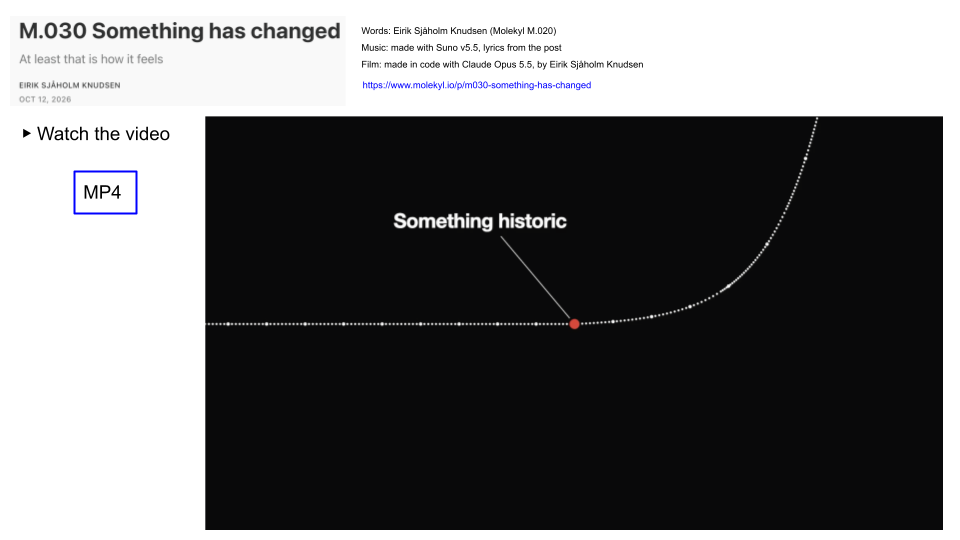
\includegraphics[width=.64\linewidth]{figures/talk/slide-23.png}}
\biopath
How can a creative explanation help people understand a scientific idea? Eirik Sj\aa holm Knudsen's \emph{Something has changed} combines human-written words, generated music and code-assisted film production \citep{knudsen2026changed}. A moving image may communicate a spatial process intuitively, but emotional force can also make uncertain mechanisms seem established.

\textbf{Exercise and result.} Explain oxygen-limited growth in ordinary language, then as a visual sequence. Identify an omission that could make the sequence biologically misleading and ask a viewer what they understood.
\comppath
\textbf{Define a rendering map.} Let $d$ be saved source data, $\phi$ rendering settings and assets, and $a=R(d,\phi)$ the resulting animation. For a normalized scalar value $u\in[0,1]$, a colour map $C:[0,1]\to[0,1]^3$ returns red, green and blue intensities. The three components encode colour, not three biological measurements.

If each frame is rescaled using its own minimum $l_t$ and maximum $h_t$, the displayed argument becomes
\[
\tilde u_t=\frac{u_t-l_t}{h_t-l_t},\qquad h_t>l_t.
\]
\textbf{Read the effect.} Even with unchanged physical value $u_t=0.5$, range $[0,1]$ gives $\tilde u_t=0.5$, while range $[0,0.5]$ gives $\tilde u_t=1$. A changing colour can therefore arise from changing scale rather than changing biology. The map must also state how it handles values outside its declared range.

\textbf{Interpretation and exercise.} Formulate the invariant: equal physical values must receive equal colours across compared frames. Specify fixed limits and test the invariant on two saved frames. Distinguish reproducible rendering from saved assets from exact replay of an external generation service; preserve the sources and revision decisions for each stage.
\sharedpath
An intuitive visual explanation and an explicit rendering invariant together protect the scientific meaning of a creative presentation.
\end{slidenotes}

\begin{slidenotes}{24}{A human response to AI change}{\href{https://vimeo.com/1234541249}{
\includegraphics[width=.34\linewidth]{figures/talk/slide-24-video.png}}\\[1.5mm]
{\small\textbf{Prof. Eirik S. Knudsen}\quad\href{https://www.molekyl.io}{www.molekyl.io}}}
\setlength{\parskip}{3pt}
\begin{tcolorbox}[colback=gray!3,colframe=gray!35,boxrule=.3pt,arc=1mm,left=2mm,right=2mm,top=1mm,bottom=1mm,before skip=2pt,after skip=3pt,fontupper=\footnotesize]
\textbf{Transcript of the narration.} \emph{Punctuation and paragraph breaks edited.}

Something has changed. At least that's how it feels. It began as a small itch in the fall. It became more noticeable in November and December. Now it's impossible to ignore. The feeling that we are in the middle of something historic. Something I will look back at, asking what I thought at this exact moment, why I did as I did. Something that makes me want to drop everything, to fully catch the wave, or to move to a remote farm without internet.

You might think this something is AI. It isn't. It's that feeling created by the state of AI. That feeling of shock and awe, fear and joy, of optimism and pessimism. Other things can evoke each of these. With AI, it's all at once. Strong, weird and unpredictable. So what do I do? I do it all. I humanize and automate. I slow down and speed up. I connect and disconnect. Which does and doesn't make sense, because AI is a contradiction.

It's alive and it's dead. It's present and it's distant. It's here and it isn't. All this makes everything easy and hard at the same time. But the feeling is clear, strong, unmissable. If you have it, you know what I mean. If you don't, enjoy the bliss while it lasts.
\end{tcolorbox}
\biopath
What changes for the person doing the work? The film's shock, hope and ambivalence concern human experience \citep{knudsen2026changed}. In a clinic, faster drafting could free time for conversation or increase checking. The patient's concerns may differ from the professional's enthusiasm.

\textbf{Exercise and result.} Explain one activity you would delegate and one in which your participation has meaning. Name an observation that could change your view.
\comppath
\textbf{Define the measured effort.} Let $T_g,T_r,T_v$ be generation, review and revision times, all in minutes for one accepted output. Total effort is
\[
T=T_g+T_r+T_v.
\]
\textbf{Read the sum.} Each term counts a different part of the workflow. An invented comparison gives $5+1+1=7$ minutes initially and $1+5+3=9$ with assistance: faster generation can coexist with greater total effort. This simple sum assumes sequential, non-overlapping work; elapsed time needs a different account if activities overlap.

\textbf{Exercise and interpretation.} Define separate comprehension score $C$ and emotional-response score $E$, including their scales. For assigned film and transcript groups, compare mean $C$ on the same questions and report $E$ separately. Explain why a difference in $E$ alone cannot establish a difference in $C$.
\sharedpath
Human purposes determine which outcomes matter; explicit time and outcome variables make a capability or educational claim testable.
\end{slidenotes}

\begin{slidenotes}{25}{Synthesis and a next experiment}{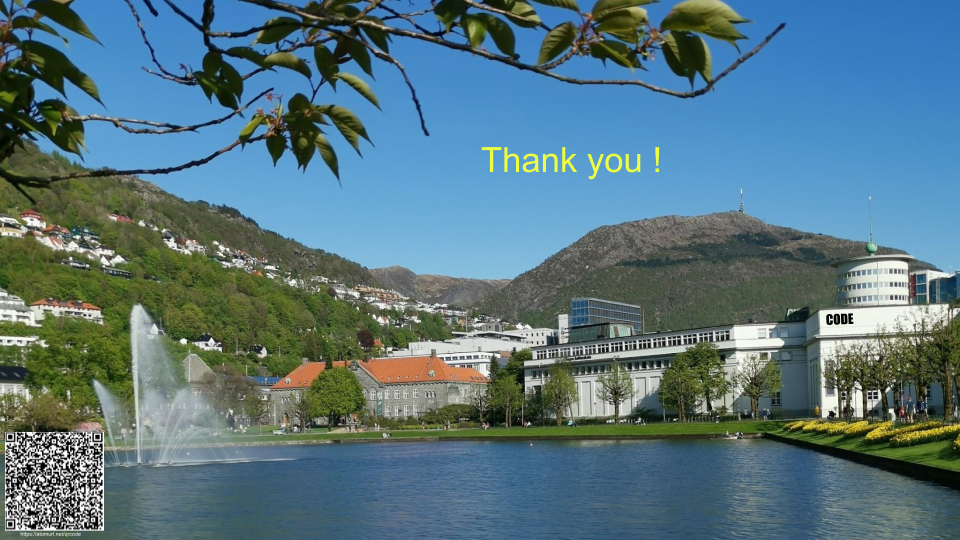
\includegraphics[width=.64\linewidth]{figures/talk/slide-25.png}}
\biopath
What does a positive result mean for a person? In a hypothetical 10,000-person population with 1\% prevalence and 90\% sensitivity and specificity, expect 90 true positives and 990 false positives. About 8.3\% of positive results therefore correspond to disease. Explain this with people counted, then discuss why action also depends on consequences and further evidence.

\textbf{Exercise and result.} Explain the positive result without starting with a formula. Ask a colleague to describe it back and identify one observation that would change your interpretation.
\comppath
\textbf{Define the probabilities.} Let $D$ be the event that disease is present and $+$ a positive test. Prevalence is $\pi=P(D)$, sensitivity $\mathrm{Se}=P(+\mid D)$ and specificity $\mathrm{Sp}=P(-\mid\neg D)$. The vertical bar means ``given''; $\neg D$ means absence of disease. Bayes' rule gives
\[
P(D\mid+)=\frac{\mathrm{Se}\,\pi}
{\mathrm{Se}\,\pi+(1-\mathrm{Sp})(1-\pi)}.
\]
\textbf{Read the fraction.} The numerator is the probability of disease and a positive test. The denominator adds true-positive and false-positive probabilities, giving $P(+)$. Their ratio is the fraction of positives with disease, or PPV. It is defined only when the denominator is positive. At $\pi=0.01$ and $\mathrm{Se}=\mathrm{Sp}=0.9$, it is $0.009/(0.009+0.099)=1/12$.

\textbf{Exercise and interpretation.} For a decision probability $p$ and stipulated costs $C_{FP}=1$, $C_{FN}=4$, compare expected losses $1-p$ and $4p$. Derive $p>0.2$, with a tie at equality. Distinguish group prevalence $\pi$ from probability $p$ given the evidence for a decision. \coursenotebook{15_ppv_and_decisions.ipynb}{Notebook 15} connects counts, conditional probabilities and the action boundary.
\sharedpath
Population counts convey clinical meaning; conditional probabilities and explicit losses establish the calculation and the assumptions connecting prediction to action.
\end{slidenotes}
\endgroup
